\chapter{Valiable Pipelined CMAの概要}
{
\label{chap:vpcma}
本章では、本論文で対象としているアーキテクチャであるValiable Pipelined CMAの概要を説明する。
\section{CMAの概要}
\label{sec:about_cma}
CMAは主にバッテリー駆動の組み込みシステムにおけるマルチメディア処理を行うアクセラレータとして提案された。\cite{cma_micro}マルチメディア処理の特性として一定時間内に一定量のデータ処理を行うことが要求される。一方でこれらの処理を要求されている時間よりも早く完了させることによって得られる利益は少ない。したがって、処理時間を調整して不必要な消費電力を削減することが可能であり、バッテリー使用時間を長くすることにつながる。CMAアーキテクチャでは主に以下のコンセプトによって消費電力の削減を図っている。

\begin{itemize}
\item PEアレイからクロックツリーとレジスタを除去し、完全な組み合わせ回路として構成する
\item 各PEの演算やデータパスの動的な再構成を行わない
\end{itemize}

一般的なDRPでは、動的な再構成のために各PEにおいてレジスタを持ち、クロックが供給される。したがってクロックツリーと動的な再構成のための処理において大きな電力を消費する。一方でCMAではPEにはレジスタやクロックツリーは存在せず組み合わせ回路のみで構成している。このような構成を採用することにより上記のコンセプトを実現している。

初代試作機のCMA-1からCCSOTBまではPE\_ARRAYへのクロック供給とレジスタはなかった。そこでPE\_ARRAYをパイプライン分割することによる発生するオーバーヘッドと性能の関係が研究されValiable Pipelined CMAが提案された。\cite{vpcma}パイプライン分割のためにPE\_ARRAYに追加されたパイプラインレジスタにおける消費電力は全体の数\%であり、クロックツリーでの消費電力は最大で全体の60\%を占めている。
このようにパイプライン分割による電力増加がある、一方で高いスループット向上が得られ全体としてはエネルギー効率が改善されている。エネルギー効率は最大で96\%向上したと報告されている。
% ところが、パイプライン分割による性能向上の影響が勝り、最大で96\%のエネルギー効率を実現できることが確認された。

% %DRPとCMAの構成図
% \begin{figure}[h]
%   \begin{center}
%     \begin{tabular}{c}

%       % 1
%       \begin{minipage}{0.33\hsize}
%         \begin{center}
%           %\includegraphics[clip, width=4.5cm]{./fig/DRP.eps}
%           \hspace{1.6cm} (a)DRPにおけるPEの構成
%         \end{center}
%       \end{minipage}

%       % 2
%       \begin{minipage}{0.33\hsize}
%         \begin{center}
%           %\includegraphics[clip, width=4.5cm]{./fig/PE.eps}
%           \hspace{1.6cm} (b)CMAにおけるPEの構成
%         \end{center}
%       \end{minipage}


%     \end{tabular}
%     \caption{DRPとCMAにおける構成の違い}
%     \label{fig:DRP_vs_CMA}
%   \end{center}
% \end{figure}


\section{CMAの構成}
\label{sec:about_cma}
CMAを構成する要素とそれらの動作を説明していく。CMAは主に以下の要素で構成されている。
\begin{itemize}
\item PE\_ARRAY    
\item $\mu$コントローラ
\item コンフィギュレーションレジスタ
\item 定数値レジスタ
\end{itemize}

\subsection{PE\_ARRAY}
\label{subsec:pe_array}
図\ref{fig:pe_array}にPE\_ARRAYの構成を示す。12列$\times$8行のPEとそれらの相互接続、パイプライン分割のためのレジスタから構成されている。パイプラインレジスタはPEの行と行の間に置かれている。パイプラインの動作に関しては\ref{subsec:pipeline}節で詳しく説明する。すでに述べているようにPEに対してはクロックの分配をしない、一方でパイプラインレジスタへはクロックが分配されている。ただし、可変パイプラインであるため使用しないパイプラインレジスタに対してはクロックゲーティングを行うことで不要な消費電力が発生しないようにしている。このPE\_ARRAY全体はおよそ0.5V$\sim$1.2Vの電源電圧で動作する。PE\_ARRAYの入出力は南方向のみであり、入力にはfetchレジスタが、出力にはgatherレジスタが接続されている。つまり、fetchレジスタ、gatcherレジスタともにPE\_ARRAYの0行目の0番から11番までの列と接続されている。そのためデータ幅は25bit$\times$12である。fetchレジスタにデータを書き込むことでPE\_ARRAYでの演算が開始し、適切なタイミングでgatherレジスタにデータを取り込む。\\

\begin{figure}[p]
\centering
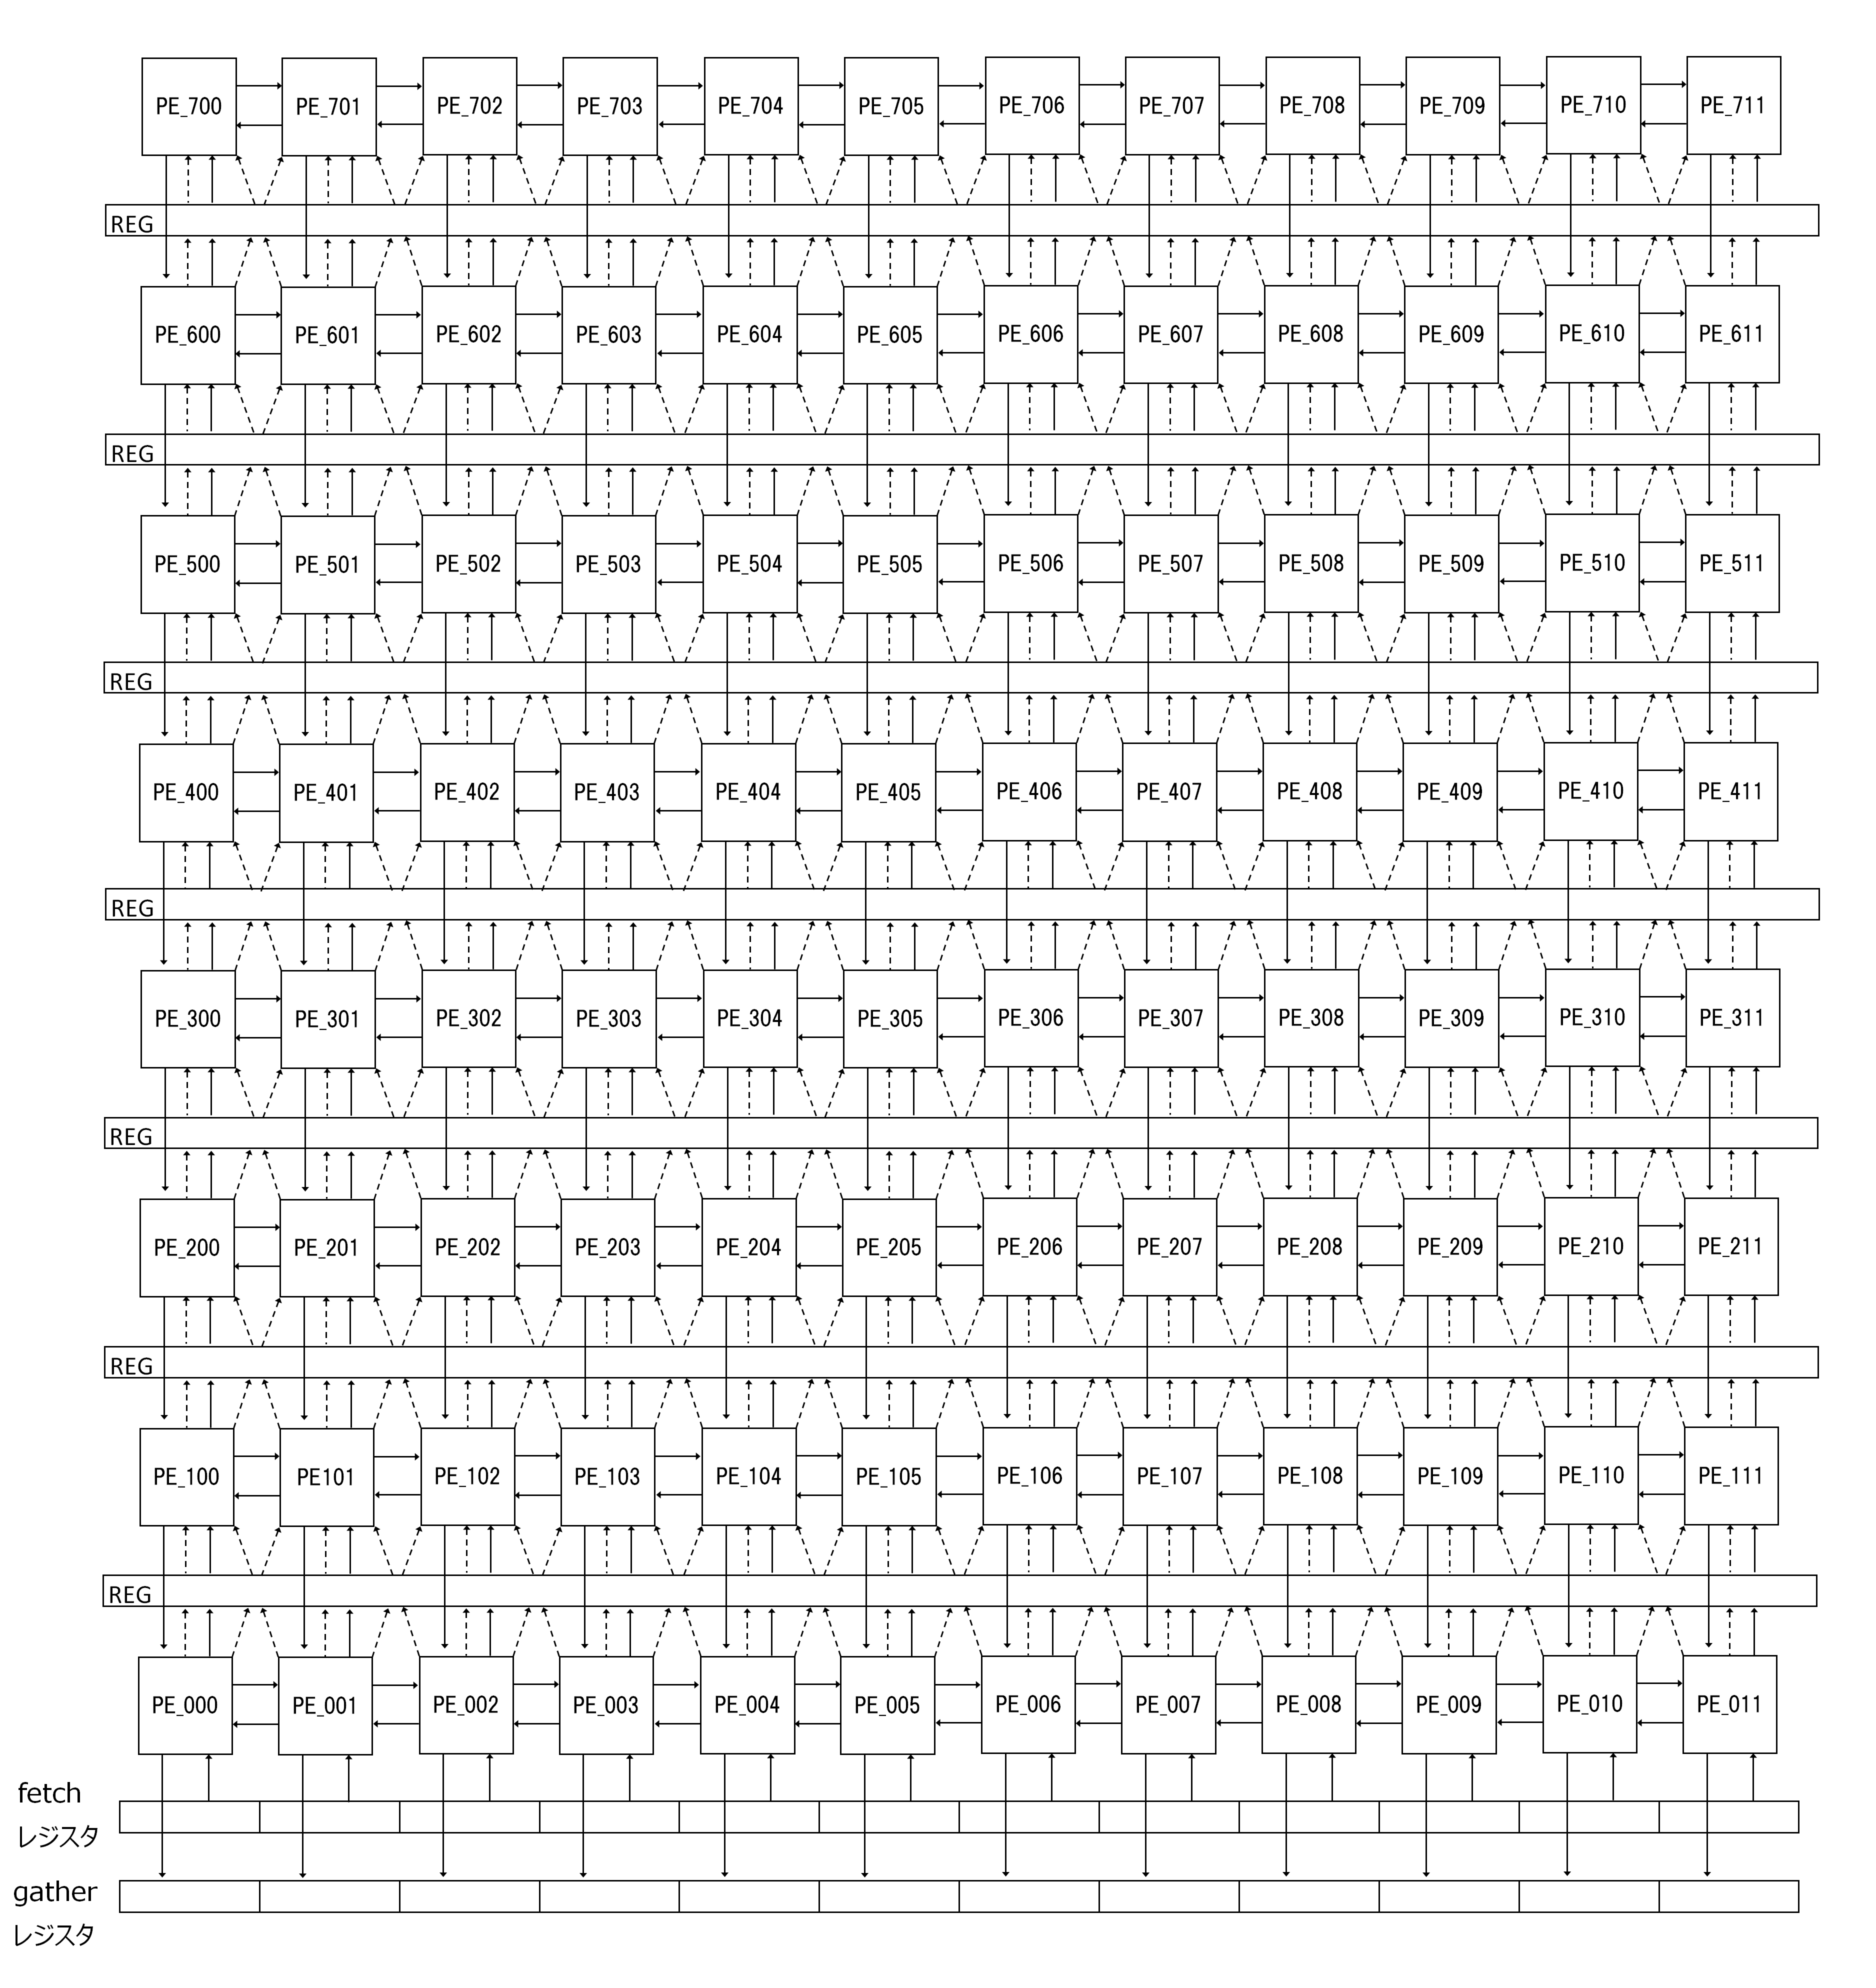
\includegraphics[scale=0.15]{./chap4/fig/PE_ARRAY.eps}
\caption{PE\_ARRAYの構成}
\label{fig:pe_array}
\end{figure}

PEの構成を図\ref{fig:pe}に示す。各PEは以下の要素から構成されている。
\begin{itemize}
\item ALU(Arithmetic Logic Unit)
\item ALUへの入力のセレクタ
\item SE(Switch Element)
\end{itemize}

\begin{figure}[h]
\centering
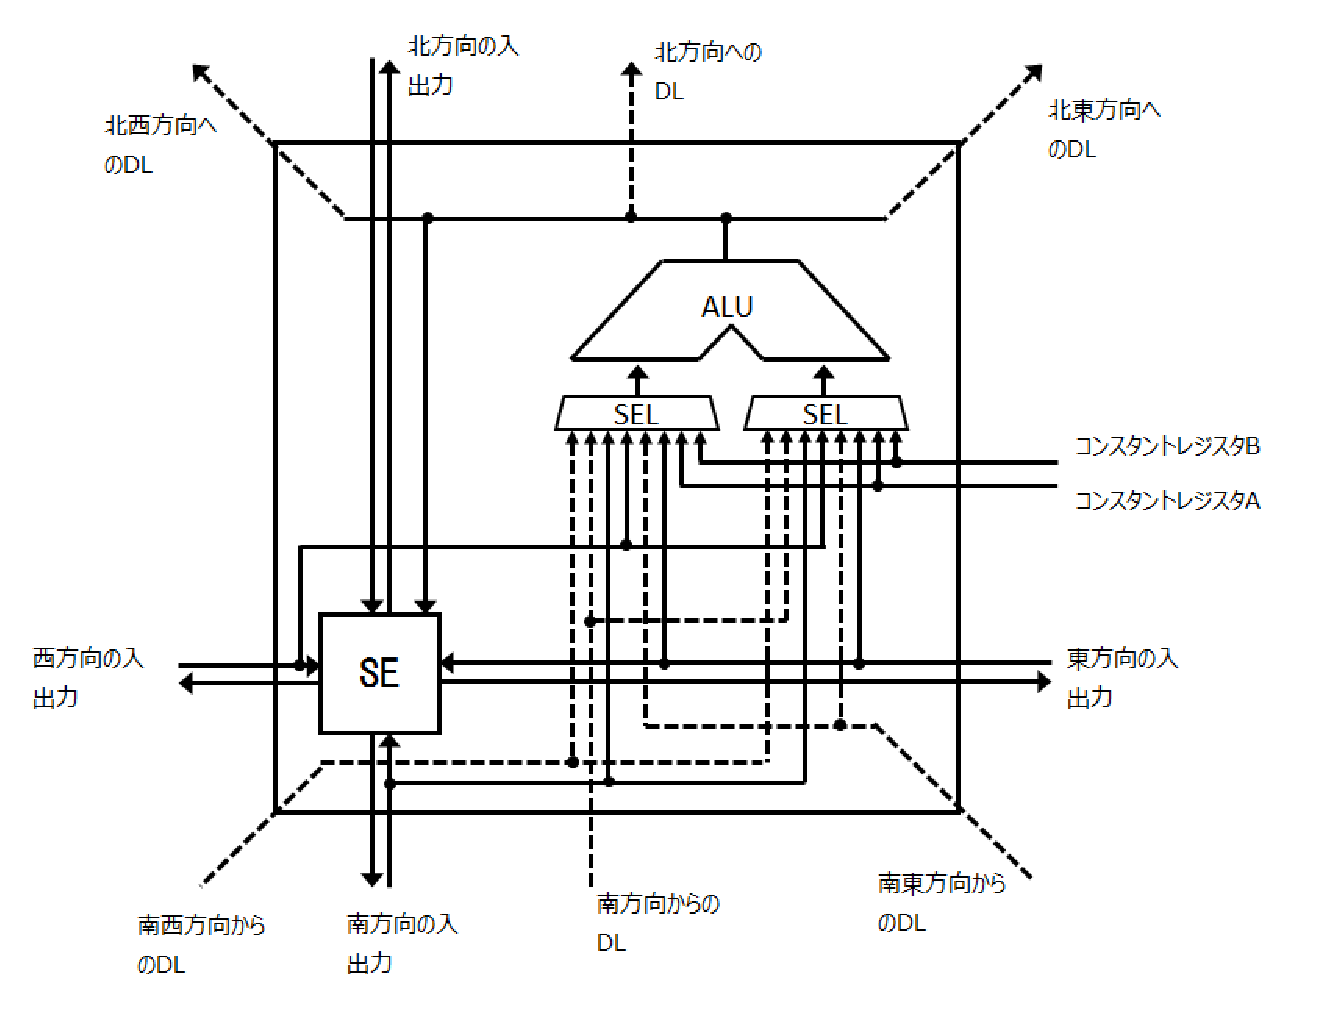
\includegraphics[scale=0.5]{./chap4/fig/PE_detail.eps}
\\ \begin{flushleft}※DL:ダイレクトリンク\end{flushleft}
\caption{PEの構成}
\label{fig:pe}
\end{figure}

ALUはデータ幅25bitの2入力1出力で演算を行う部分である。ALUの出力はSEへの入力、隣接する北方向、北東方向、北西方向のPEへのダイレクトリンクへと接続される。ダイレクトリンクとはSEを経由せずに隣接するPEへデータを送るローカルな接続である。図\ref{fig:pe}において破線で表される接続がダイレクトリンクである。ALUで使用可能な演算を表\ref{table:ALU}に示す。ただし、入力される2つのデータを$indataA$, $indataB$としている。SEは東西南北方向の隣接するPEとの相互接続を行うスイッチである。ALUへの入力のセレクタは東西南方向からの入力、南方向、南東方向、南西方向からのダイレクトリンク、および定数値レジスタから演算に使用するデータを選択する。図\ref{fig:pe_array}においてPE間の相互接続を見ると行をまたぐ接続ー3つのダイレクトリンク、北方向の出力と出力、南方向からの入力ーはパイプラインレジスタを経由することがわかる。ただし、南方向への出力、北方向からの入力はパイプラインレジスタを経由していない。

\begin{table}[h]
\centering
\caption{ALUで使用可能な演算の一覧}
\label{table:ALU}
\begin{tabular}{|c|l|} \hline
演算名 & 出力される演算結果 \\ \hline \hline
NOP & 0 \\ \hline
ADD &  $indataA$ + $indataB$\\ \hline
SUB &  $indataA$ - $indataB$\\ \hline
MULT & $indataA$ $\times$ $indataB$ \\ \hline
SL & $indataA$を$indataB$ビット左へシフト \\ \hline
SR &  $indataA$を$indataB$ビット右へ論理シフト\\ \hline
SRA & $indataA$を$indataB$ビット右へ算術シフト \\ \hline
\multirow{2}{*}{SEL} & if ($indataA$のMSB==1) $indataA$ \\
					&  else \hspace{89pt} $indataB$ \\ \hline
CAT & $indataA$ \\ \hline
NOT & NOT $indataA$ \\ \hline
AND &  $indataA$ AND $indataB$\\ \hline
OR &  $indataA$ OR $indataB$\\ \hline
XOR & $indataA$ XOR $indataB$ \\ \hline
\multirow{2}{*}{EQL} & if ($indataA$==$indataB$) $indataA$ \\
					&  else \hspace{80pt} $indataB$ \\ \hline
\multirow{2}{*}{GT} & if ($indataA$ $>$ $indataB$) $indataA$ \\
					&  else \hspace{80pt} $indataB$ \\ \hline
\multirow{2}{*}{LT} & if ($indataA$ $<$ $indataB$) $indataA$ \\
					&  else \hspace{80pt} $indataB$ \\ \hline
\end{tabular}
\end{table}

\subsection{$\mu$コントローラ}
\label{subsec:micro_controller}
$\mu$コントローラは固定長16bitの命令を実行する小さなプロセッサであり、PE\_ARRAYとデータメモリの間のデータ転送などを行う。$\mu$コントローラには表\ref{table:iset}に示す命令セットを持つ。$\mu$コントローラは25bitの汎用レジスタを16個持っている。表\ref{table:iset}中のrd,rsはレジスタを表す。n,imm,adr, X, X1, X2は即値であり、左の()で囲まれた数値はビット数である。

\begin{table}[p]
\begin{center}
\caption{$\mu$コントローラの命令セット}
\label{table:iset}
\begin{tabular}{|l|l|l|} \hline
オペコード & オペランド & 命令の意味 \\ \hline
NOP & & \\ \hline
ADD & rd, rd & rd $\leftarrow$rd + rs \\ \hline
SUB & rd, rs & rd $\leftarrow$rd - rs \\ \hline
MV & rd, rs & rd $\leftarrow$ rs\\ \hline
DONE & & プログラムの終了を示す\\ \hline
DELAY & n(4) & G.Rにデータを取り込むまでの遅延サイクル数nを指定する \\ \hline
LDI & rd, imm(8) & rd $\leftarrow$  imm \\ \hline
ADDI & rd, imm(8) & rd $\leftarrow$ rd  + imm \\ \hline
BEZ & rd, imm(8) & if (rd==0) pc $\leftarrow$ pc + imm \\ \hline
\multirow{2}{*}{BEZD} & \multirow{2}{*}{rd, imm(8)} & rd $\leftarrow$ rd - 1 \\
& &  if (rd==0) pc $\leftarrow$ pc + imm \\ \hline
BNZ & rd, imm(8) & if (rd!=0) pc $\leftarrow$ pc + imm \\ \hline
\multirow{2}{*}{BNZD} & \multirow{2}{*}{rd, imm(8)} &  rd $\leftarrow$ rd - 1\\ 
& & if (rd!=0) pc $\leftarrow$ pc + imm \\ \hline
& & データメモリからF.Rへのデータをロードする際の設定を行う \\
LD\_SET & adr(8), X(4) &  adr: データメモリのロード開始アドレスを指定 \\
& & X:データマニピュレータのテーブル番号を指定\\ \hline
& & G.Rからデータメモリへデータをストアする際の設定を行う \\
ST\_SET & adr(8) , X(4) &  adr: データメモリのストア開始アドレスを指定\\ 
& & X: データマニピュレータのテーブル番号を指定\\ \hline
\multirow{6}{*}{LDST\_ADD} &  \multirow{6}{*}{X1(4), X2(4)} & データメモリのロード開始アドレスからX1個のデータを \\
& & 						F.Rレジスタへロードする \\
& & 						ロード開始アドレスにX1を加算する \\
& & 						 nサイクルの遅延の後G.Rからデータメモリのストア開始アドレス \\
& & 						からX2個のデータをストア \\
& & 						ストア開始アドレスをX2加算する\\ \hline
\end{tabular}
\end{center}
※F.R: fetchレジスタ G.R: gatherレジスタ pc: プログラムカウンタ
\end{table}

データメモリのロードとストアの動作について説明する。$\mu$コントローラにおけるデータメモリは12個のバンクに分割されている。そのため同時に25bitのデータを最大で12個読み書きすることが可能である。これはPE\_ARRAYが12列で構成されているためである。データメモリからロードしたデータをfetchレジスタのどの列へ書き込みを行うかの対応付けを行うのがデータマニピュレータである。同様にgatherレジスタのどの位置からデータを読み込み、データメモリへストアするかの対応付けをデータマニピュレータが行う。

表\ref{table:ldtbl}をデータマニピュレータのテーブルとして指定した時のロード時の様子を図\ref{fig:LD_dmanu}に示す。マスク部分はその列番号についてロードを行うか否かを表している。0の列のfetchレジスタには書き込みをせず、1の列のfetchレジスタに対して書き込みを行う。fetchレジスタへ書き込みを行う列はデータメモリのアドレスを指定する必要がある。LDテーブルは各列についてロード開始アドレスに対するオフセットを持っており、これによって読み込むデータのアドレスを指定している。この例ではロードするデータの数は4個であるため、1回のロードが終わるとロード開始アドレスは4加算され次のロード処理に備える。この機構によりPE\_ARRAYとデータメモリのやり取りを柔軟に行うことが可能となる。

\begin{table}[h]
\centering
\caption{LDテーブルの例}
\label{table:ldtbl}
\begin{tabular}{|c|c|c|c|c|c|c|c|c|c|c|c|c|} \hline
fetchレジスタの列番号 & 0 & 1 & 2 & 3 & 4 & 5 & 6 & 7 & 8 & 9 & 10 & 11 \\ \hline \hline 
マスク部分 & 1 & 0 & 0 & 1 & 0 & 0 & 1 & 0 & 0  & 1 & 0 & 0 \\ \hline
ロード開始アドレスに & \multirow{2}{*}{0x0} & \multirow{2}{*}{0x0} & \multirow{2}{*}{0x0} & \multirow{2}{*}{0x1} & \multirow{2}{*}{0x0} & \multirow{2}{*}{0x0} & \multirow{2}{*}{0x2} & \multirow{2}{*}{0x0} & \multirow{2}{*}{0x0} & \multirow{2}{*}{0x3} & \multirow{2}{*}{0x0} & \multirow{2}{*}{0x0} \\ 
対するオフセット & & & & & & & & & & & & \\ \hline
\end{tabular}
\end{table}

\begin{figure}[]
\centering
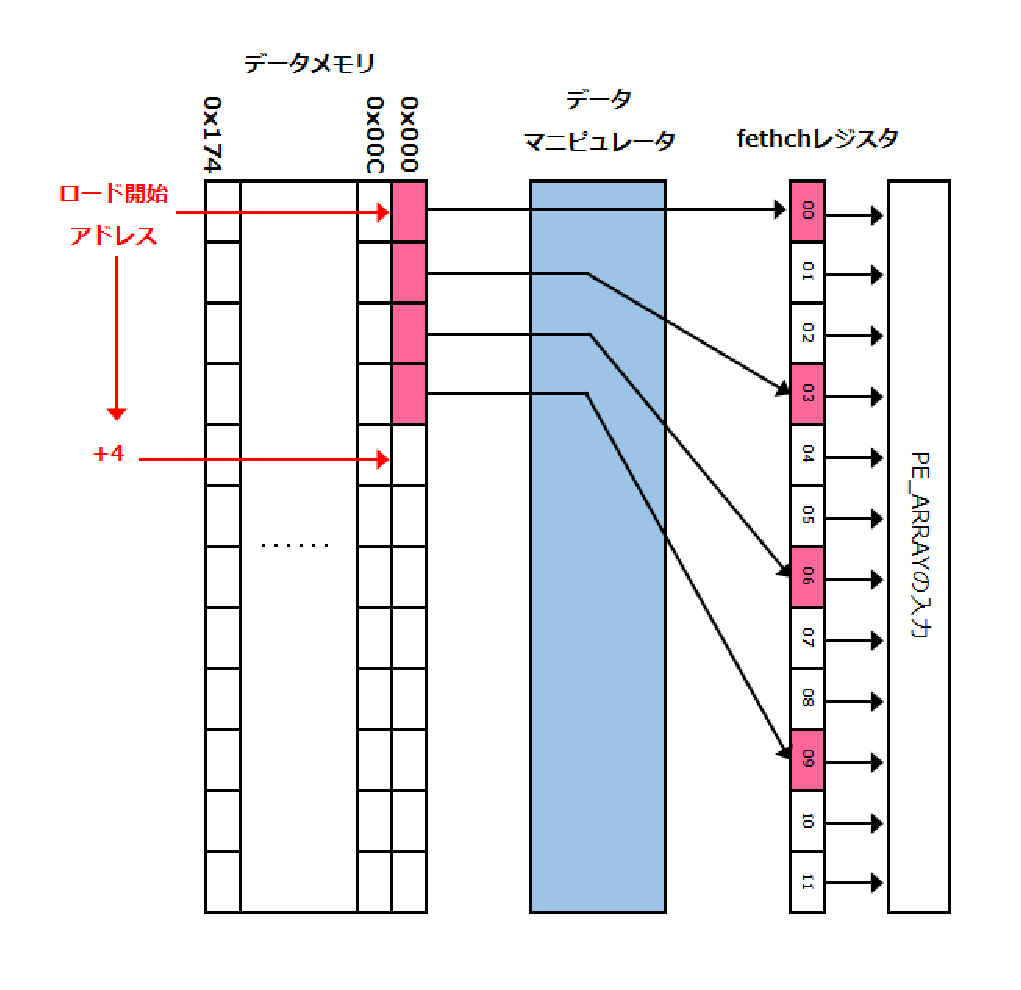
\includegraphics[width=8cm]{./chap4/fig/LD_dmanu.eps}
\caption{ロード時のデータマニピュレータ様子}
\label{fig:LD_dmanu}
\end{figure}


gatherレジスタへ演算結果を取り込みデータメモリへのストアが行われるのは表\ref{table:iset}で見たようにデータメモリからfetchレジスタへデータをロードしてから指定したサイクル数遅延してから行われる。これはPE\_ARRAYは大規模な組み合わせ回路であり計算結果が出力されるまでに長い時間が必要であり、$\mu$コントローラの1クロックサイクル以内に演算を完了できない場合が殆どだからである。ストアの動作に関しても同様にデータマニピュレータの対応付けによって指定した列の出力のみをデータメモリへ書き込み、書き込んだデータ数の分だけストア開始アドレスが加算される。表\ref{table:sttbl}をデータマニピュレータのテーブルとして指定した時のストア時の様子を図\ref{fig:ST_dmanu}に示す。この例ではストアするデータの数は2個であるため、1回のストアが終わるとストア開始アドレスは2加算される。

\begin{table}[h]
\centering
\caption{STテーブルの例}
\label{table:sttbl}
\begin{tabular}{|c|c|c|c|c|c|c|c|c|c|c|c|c|} \hline
gatherレジスタの列番号 & 0 & 1 & 2 & 3 & 4 & 5 & 6 & 7 & 8 & 9 & 10 & 11 \\ \hline \hline
マスク部分 & 1 & 0 & 0 & 0 & 0 & 0 & 1 & 0 & 0  & 0 & 0 & 0 \\ \hline
ストア開始アドレスに & \multirow{2}{*}{0x0} & \multirow{2}{*}{0x0} & \multirow{2}{*}{0x0} & \multirow{2}{*}{0x0} & \multirow{2}{*}{0x0} & \multirow{2}{*}{0x0} & \multirow{2}{*}{0x1} & \multirow{2}{*}{0x0} & \multirow{2}{*}{0x0} & \multirow{2}{*}{0x0} & \multirow{2}{*}{0x0} & \multirow{2}{*}{0x0} \\ 
対するオフセット & & & & & & & & & & & & \\ \hline
\end{tabular}
\end{table}

\begin{figure}[h]
\centering
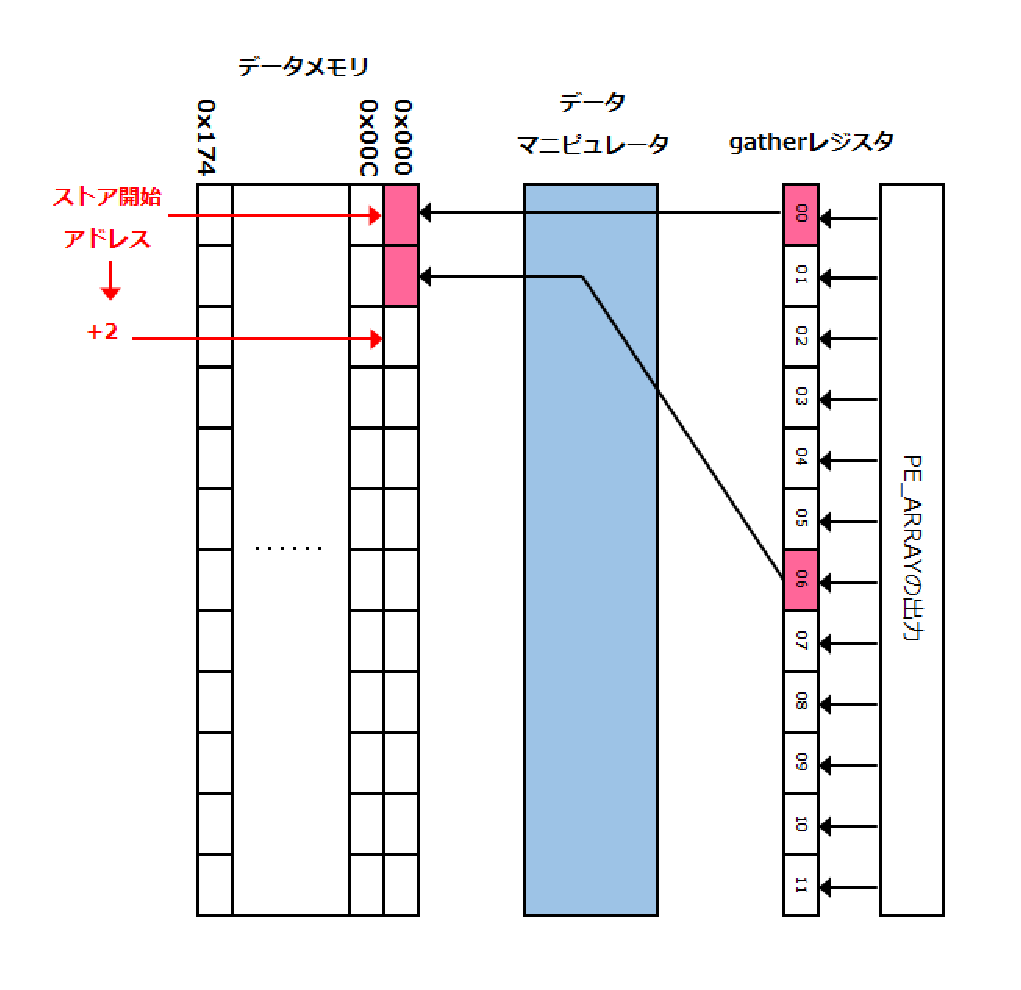
\includegraphics[width=8cm]{./chap4/fig/ST_dmanu.eps}
\caption{ストア時のデータマニピュレータの様子}
\label{fig:ST_dmanu}
\end{figure}


\subsection{コンフィギュレーションデータ}
\label{subsec:config_data}

コンフィギュレーションデータとはPE\_ARRAY内にある各PEとパイプラインレジスタの構成情報を指定するものである。PE\_ARRAYの外部にコンフィギュレーションレジスタが配置されており、そこからPE\_ARRAYへ送信される。使用するパイプラインレジスタをコンフィギュレーションデータに含めることでアプリケーションごとに可変なパイプライン段数を使用することが可能となる。すでに述べているようにアプリケーション実行を通してコンフィギュレーションデータは動的に変化することはない。

\section{演算のマッピングとアプリケーション実行の様子}
\label{sec:mapping}
PE\_ARRAYにアプリケーションをマッピングして実行する様子を説明する。前半ではパイプライン分割を行わない場合を、後半ではパイプライン分割を行った場合の動作を説明する。例としてRGB24bitのグレースケールを行うアプリケーションを用いる。PE\_ARRAYは12列あるがここでは簡略化のためにPE\_ARRAYのはじめの2列のみを示す。演算のマッピングされたPEとその相互接続の様子を図\ref{fig:mapping}に示す。各PEにマッピングされた演算が記されている。何も書かれたいない2つのPEはスイッチとしてのみ利用されていて、ALUは使用されない。

\begin{figure}[p]
\centering
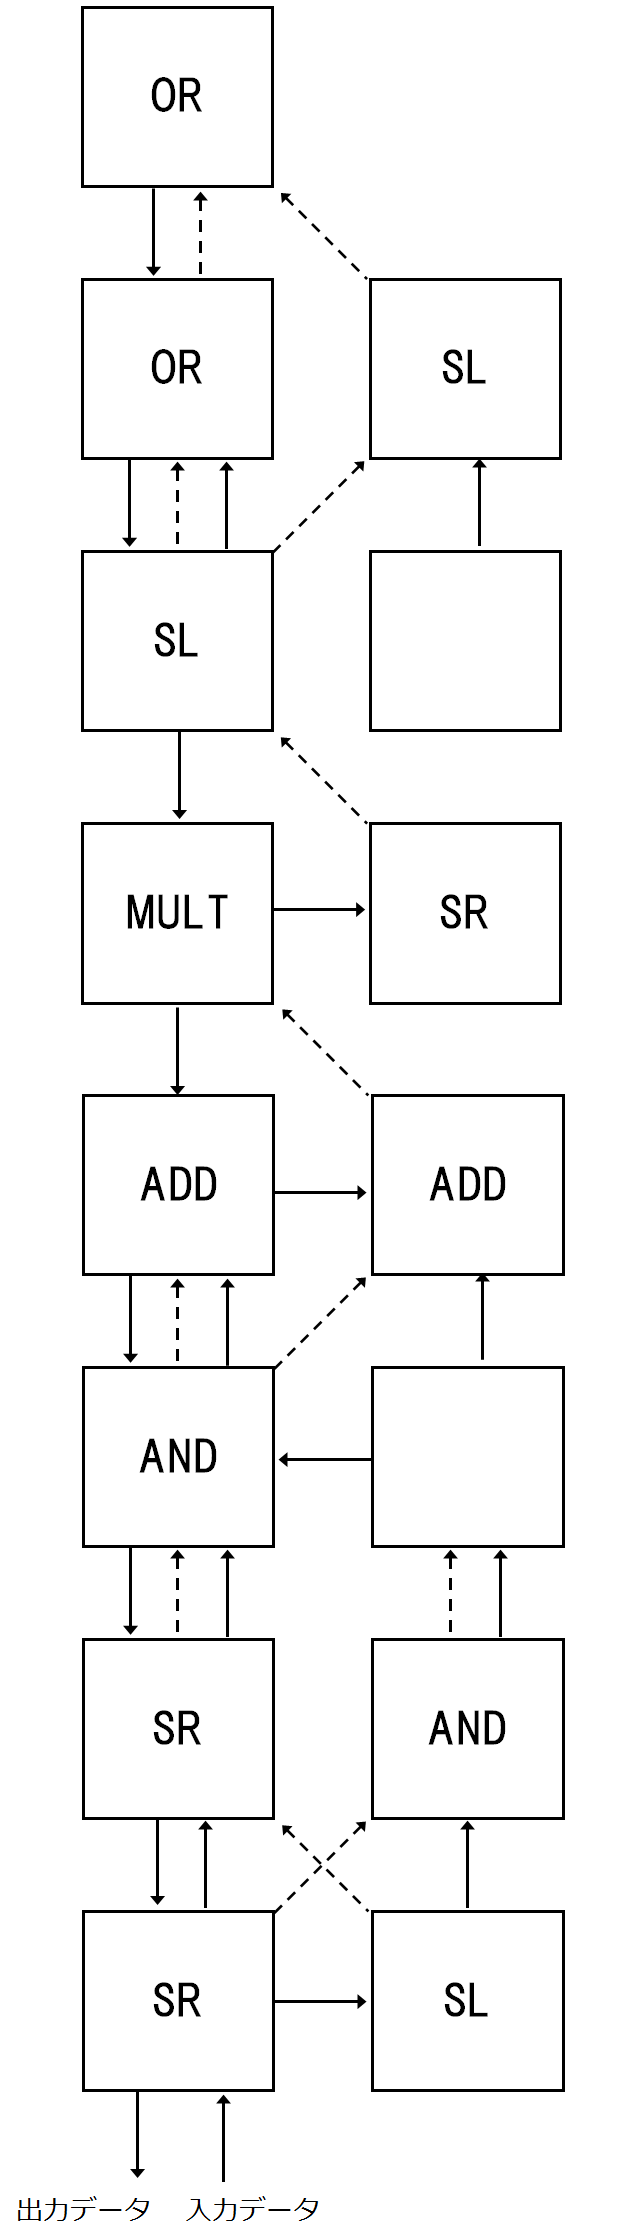
\includegraphics[width=4cm]{./chap4/fig/mapping.eps}
\caption{アプリケーションのマッピング例:}
\label{fig:mapping}
\end{figure}

次に$\mu$コントローラにおけるアプリケーション実行の様子を説明する。比較のためにパイプライン分割しない場合と、パイプライン分割する場合で同じクロックサイクル、つまり同じ周波数で動作する例を考える。

\subsection{パイプライン分割をしない場合}
\label{subsec:not_pipeline}
$\mu$コントローラにおける命令コードを以下に示す。この命令コードを実行したときの様子を図\ref{fig:not_pipelined_look}に示す。
\begin{itembox}[l]{パイプライン分割しない場合の命令コード}
\begin{verbatim}
        DELAY 7
        LDI r3,#8
        SET_LD #0,#6
        SET_ST #0x30,#6
LP:     LDST_ADD #0,#0
        NOP
        NOP
        NOP
        NOP
        NOP
        BNZD r3,LP
        DONE
\end{verbatim}
\end{itembox}

データメモリの0x0番地からデータを6個ロードして、データメモリの0x30番地にデータを6個ストアすることを8回ループすることを示している。演算終了まで7クロックサイクル遅延してからストアを行っている。演算結果をgatherレジスタに取り込むまでは新しいデータをPE\_ARRAYに入力して演算を開始させることができないのでそれまでNOP命令を挿入している。

\begin{figure}[h]
\centering
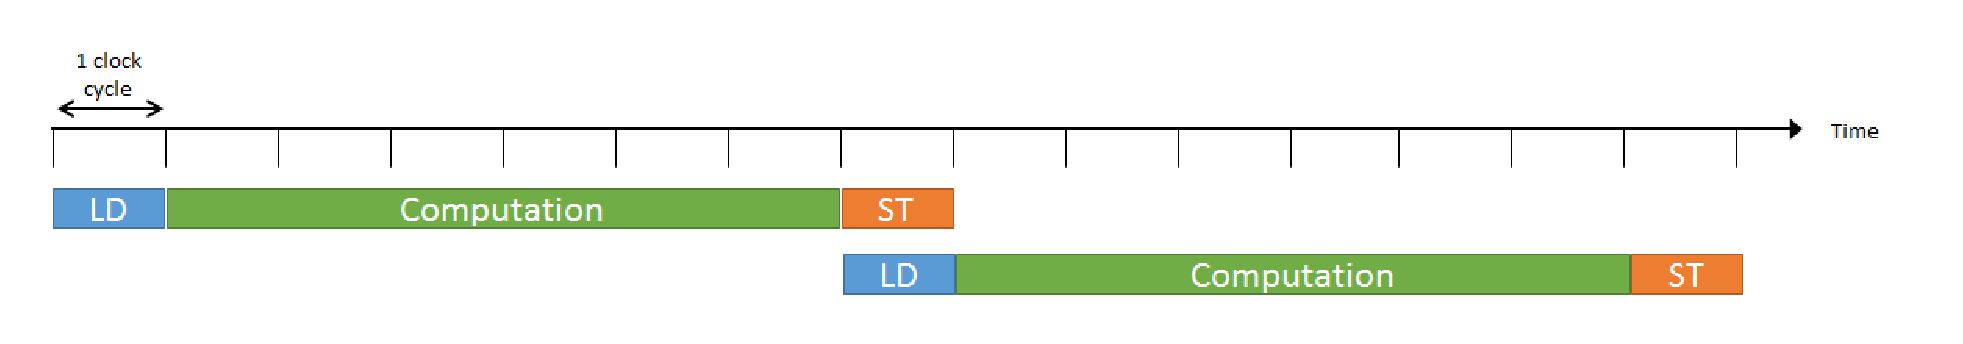
\includegraphics[width=12cm]{./chap4/fig/not_pipelined_look.eps}
\caption{パイプライン分割しない場合の実行の様子}
\label{fig:not_pipelined_look}
\end{figure}

\subsection{パイプライン分割をする場合}
\label{subsec:pipeline}
ここではすべてのパイプラインレジスタを用いる、すなわちパイプライン段数8の場合を考える。$\mu$コントローラにおける命令コードを以下に示す。この命令コードを実行したときの様子を図\ref{fig:pipelined_look}に示す。
\begin{itembox}[l]{パイプライン分割しない場合の命令コード}
\begin{verbatim}
        DELAY 7
        LDI r3,#8
        SET_LD #0,#6
        SET_ST #0x30,#6
LP:     LDST_ADD #0,#0
        BNZD r3,LP
        DONE
\end{verbatim}
\end{itembox}

\begin{figure}[h]
\centering
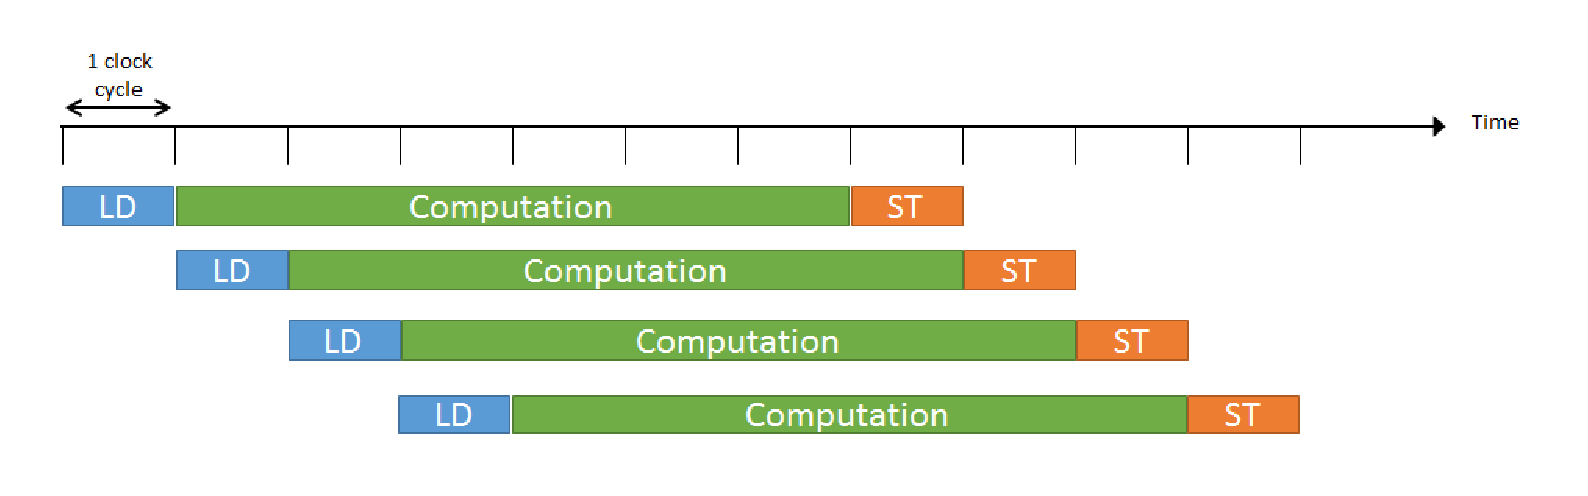
\includegraphics[width=12cm]{./chap4/fig/pipelined_look.eps}
\caption{パイプライン分割する場合の実行の様子}
\label{fig:pipelined_look}
\end{figure}

パイプライン分割しない場合の図\ref{fig:not_pipelined_look}と比べて各パイプラインステージで演算をオーバーラップさせて実行できることがわかる。

}
